% Für Bindekorrektur als optionales Argument "BCORfaktormitmaßeinheit", dann
% sieht auch Option "twoside" vernünftig aus
% Näheres zu "scrartcl" bzw. "scrreprt" und "scrbook" siehe KOMA-Skript Doku
\documentclass[12pt,a4paper,titlepage,headinclude,bibtotoc]{scrartcl}


%---- Allgemeine Layout Einstellungen ------------------------------------------

% Für Kopf und Fußzeilen, siehe auch KOMA-Skript Doku
\usepackage[komastyle]{scrpage2}
\pagestyle{scrheadings}
\setheadsepline{0.5pt}[\color{black}]
\automark[section]{chapter}


%Einstellungen für Figuren- und Tabellenbeschriftungen
\setkomafont{captionlabel}{\sffamily\bfseries}
\setcapindent{0em}


%---- Weitere Pakete -----------------------------------------------------------
% Die Pakete sind alle in der TeX Live Distribution enthalten. Wichtige Adressen
% www.ctan.org, www.dante.de

% Sprachunterstützung
\usepackage[ngerman]{babel}

% Benutzung von Umlauten direkt im Text
% entweder "latin1" oder "utf8"
\usepackage[utf8]{inputenc}

% Pakete mit Mathesymbolen und zur Beseitigung von Schwächen der Mathe-Umgebung
\usepackage{latexsym,exscale,stmaryrd,amssymb,amsmath}

% Weitere Symbole
\usepackage[nointegrals]{wasysym}
\usepackage{eurosym}

% Anderes Literaturverzeichnisformat
%\usepackage[square,sort&compress]{natbib}

% Für Farbe
\usepackage{color}

% Zur Graphikausgabe
%Beipiel: \includegraphics[width=\textwidth]{grafik.png}
\usepackage{graphicx}

% Text umfließt Graphiken und Tabellen
% Beispiel:
% \begin{wrapfigure}[Zeilenanzahl]{"l" oder "r"}{breite}
%   \centering
%   \includegraphics[width=...]{grafik}
%   \caption{Beschriftung} 
%   \label{fig:grafik}
% \end{wrapfigure}
\usepackage{wrapfig}

% Mehrere Abbildungen nebeneinander
% Beispiel:
% \begin{figure}[htb]
%   \centering
%   \subfigure[Beschriftung 1\label{fig:label1}]
%   {\includegraphics[width=0.49\textwidth]{grafik1}}
%   \hfill
%   \subfigure[Beschriftung 2\label{fig:label2}]
%   {\includegraphics[width=0.49\textwidth]{grafik2}}
%   \caption{Beschriftung allgemein}
%   \label{fig:label-gesamt}
% \end{figure}
\usepackage{subfigure}

% Caption neben Abbildung
% Beispiel:
% \sidecaptionvpos{figure}{"c" oder "t" oder "b"}
% \begin{SCfigure}[rel. Breite (normalerweise = 1)][hbt]
%   \centering
%   \includegraphics[width=0.5\textwidth]{grafik.png}
%   \caption{Beschreibung}
%   \label{fig:}
% \end{SCfigure}
\usepackage{sidecap}

% Befehl für "Entspricht"-Zeichen
\newcommand{\corresponds}{\ensuremath{\mathrel{\widehat{=}}}}

%Fußnoten zwingend auf diese Seite setzen
\interfootnotelinepenalty=1000

%Für chemische Formeln (von www.dante.de)
%% Anpassung an LaTeX(2e) von Bernd Raichle
\makeatletter
\DeclareRobustCommand{\chemical}[1]{%
  {\(\m@th
   \edef\resetfontdimens{\noexpand\)%
       \fontdimen16\textfont2=\the\fontdimen16\textfont2
       \fontdimen17\textfont2=\the\fontdimen17\textfont2\relax}%
   \fontdimen16\textfont2=2.7pt \fontdimen17\textfont2=2.7pt
   \mathrm{#1}%
   \resetfontdimens}}
\makeatother


\begin{document}

\begin{titlepage}
\centering
\textsc{\Large Anfängerpraktikum der Fakultät für
  Physik,\\[1.5ex] Universität Göttingen}

\vspace*{4.2cm}

\rule{\textwidth}{1pt}\\[0.5cm]
{\huge \bfseries
  Versuch Kreiselpräzession\\[1.5ex]
  Protokoll}\\[0.5cm]
\rule{\textwidth}{1pt}

\vspace*{3.5cm}

\begin{Large}
\begin{tabular}{ll}
Praktikant: &  Michael Lohmann\\
% &  Felix Kurtz\\
% &  Kevin Lüdemann\\
 &  Skrollan Detzler\\
 E-Mail: & m.lohmann@stud.uni-goettingen.de\\
% &  felix.kurtz@stud.uni-goettingen.de\\
% &  kevin.luedemann@stud.uni-goettingen.de\\
 &  skrollan.detzler@stud.uni-goettingen.de\\
 Betreuer: & Martin Ochmann\\
 Versuchsdatum: & 19.05.2014\\
\end{tabular}
\end{Large}

\vspace*{0.8cm}

\begin{Large}
\fbox{
  \begin{minipage}[t][2.5cm][t]{6cm} 
    Testat:
  \end{minipage}
}
\end{Large}

\end{titlepage}

\tableofcontents

\newpage

\section{Einleitung}
\label{sec:einleitung}
Kreisel spielen gerade in der Lagebestimmung eine große Rolle.
So besitzt nahezu jedes moderne Mobiltelefon Gyrosensoren, welche mithilfe von speziell gelagerten Kreiseln funktionieren.
Aber auch in der Astronomie spielen die hier beobachteten Effekte eine große Rolle.
So bewegt sich die Erde nicht genau auf einer Ellipse, sondern ''torkelt'' (wegen der Anziehungskraft des Mondes).
Dies lässt sich analog zu Kreiseln beschreiben.

\section{Theorie}
\label{sec:theorie}
Ein Kreisel ist ein Körper, der an einer Stelle gelagert ist.
Um diese kann er sich jedoch in allen Richtungen bewegen: z.B. in x- und y-Richtung, aber er kann auch rotieren.
Man kann so also erkennen, dass er insgesamt 3 Freiheitsgrade besitzt.
Um diese zu beschreiben, verwendet man gewöhnlicherweise die eulerschen Winkel.
Mit ihnen kann man den kompletten Zustand des Systems definieren.\\
Man kann nun drei verschiedene Bewegungen des Kreisels um verschiedene Kegel (s. Abb. \ref{img:kegel}): die Nutation um den Nutationskegel, Präzession um den Gangpolkegel und eine Bewegung um den Rastpolkegel 

\begin{figure}
\includegraphics{kegel.png}
\caption{verschiedene Kegel um die ein Kreisel sich bewegen kann\label{img:kegel}}
\end{figure}

\subsection{Präzession}
Ein Kreisel, der waagerecht in der Luft hängt, ohne sich zu drehen, fällt durch die Schwerkraft nach unten.
Dreht er sich jedoch schnell genug, so beginnt er, zu rotieren. Diese Bewegung nennt man Präzession.
Sie wird durch eine Kraft ausgelöst, welche senkrecht zum Drehimpuls $\vec L$ und zu dem daraus resultierenden Drehmoment $\vec M$ wirkt.
Die Präzessionsgeschwindigkeit $\omega_p$ ist die zeitliche Änderung des Winkels $\varphi$.
hallo
\subsection{Nutation}
 
\section{Durchführung}
\label{sec:durchfuehrung}


\begin{figure}
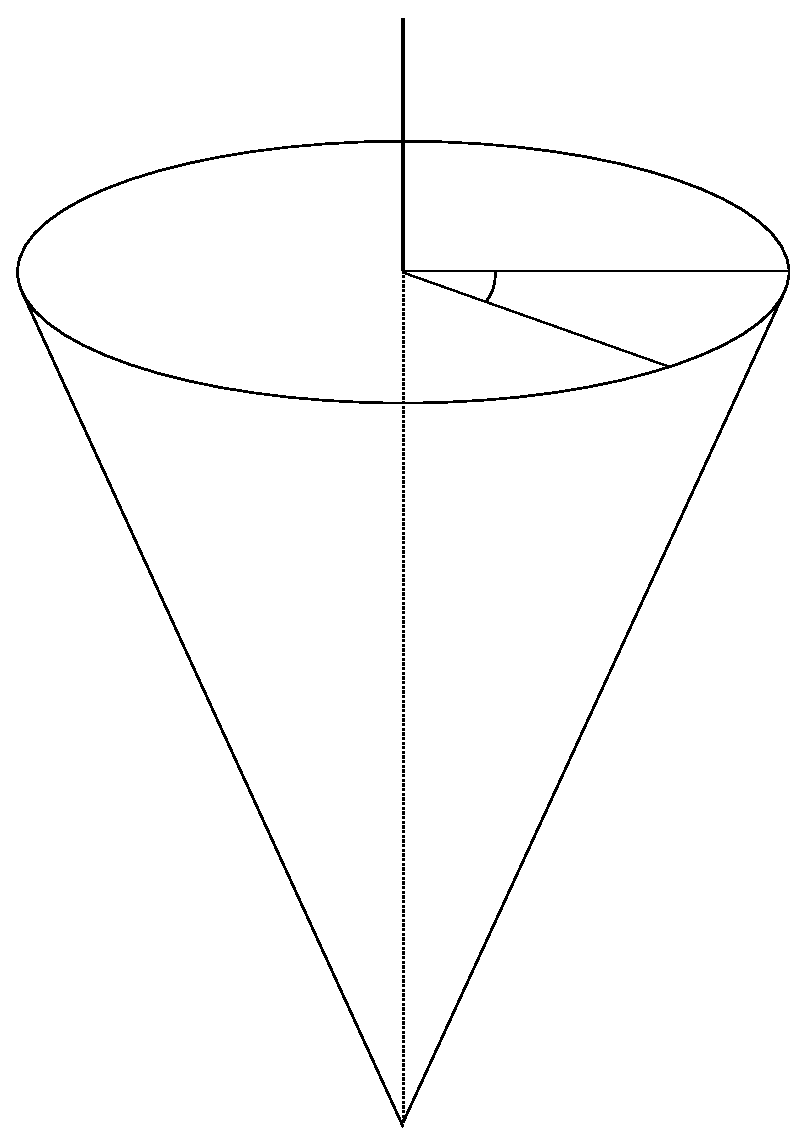
\includegraphics{bild1.eps}
\caption{Bezeichnungen der wichtigen Größen\label{img:bild1}}
\end{figure}


\section{Auswertung}
\label{sec:auswertung}

\section{Diskussion}
\label{sec:diskussion}

\end{document}
